In this chapter we prove the converse to Burkholder's theorem (Theorem \ref{thm:Burkholder}).

\begin{thm}[Bourgain]\label{thm:Bourgain}
  Let $X$ be a Banach space, and suppose that for some $p \in (1,\infty)$ the Hilbert transform $H \in \Lin(L^p(\R))$ admits a bounded $X$-valued extension.
  Then $X$ is UMD.
\end{thm}

To prove this we first need to make some reductions.
We will show that the UMD property, i.e. unconditionality of all martingale difference sequences, is equivalent to the corresponding property restricted to martingales on the dyadic filtration on the unit interval $[0,1)$: thus we don't need to consider so many martingales when establishing the UMD property.
We will also show that boundedness of the Hilbert transform implies boundedness of a corresponding Hilbert transform $H_{\T}$ on the torus $\T$, which is basically just the unit interval $[0,1)$ with addition modulo $1$.
Bourgain's painfully clever argument then relates martingales on the dyadic filtration to sequences of functions on $\T$, and bridges the gap between the Hilbert transform and UMD.

\section{The dyadic UMD property}


\begin{defn}
  For $p \in (1,\infty)$, a Banach space $X$ is said to have the \emph{dyadic $\UMD_{p}$ property} if there exists a constant $C < \infty$ such that for all $X$-valued $L^p$-bounded martingales $\mb{f}_{\bullet}$ with respect to the dyadic filtration $\mc{F}_{\bullet}$ on $[0,1)$,
  \begin{equation}\label{eq:dyadic-UMD-property}
    \Big\| \sum_{n=0}^{N} \xi_{n} d\mb{f}_{n} \Big\|_{L^p([0,1);X)} \leq C \| \mb{f}_{N}\|_{L^p([0,1);X)} \qquad \forall N \in \N.
  \end{equation}
\end{defn}

This is the same definition as that of the $\UMD_{p}$ property, but with the class of martingales restricted to martingales on the dyadic filtration.
Clearly the dyadic $\UMD_{p}$ property is implied by the standard $\UMD$ property; in this section we will prove that these two properties are equivalent.

The first step is to show that every $L^p$-bounded martingale can be approximated in $L^p$ by a martingale formed of simple functions.

\begin{lem}\label{lem:mgale-simple-approx}
  Let $X$ be a Banach space, $p \in [1,\infty)$, and $(\Omega,\mc{A},\P)$ a probability space.
  Suppose that $\mb{f}_{\bullet}$ is an $L^p$-bounded martingale on $\Omega$. 
  Then for all $\varepsilon > 0$ there exists an $X$-valued martingale $\mb{g}_{\bullet}$ on $(\Omega,\mc{A},\P)$ such that each $\mb{g}_{n}$ is simple, with
  \begin{equation*}
    \|d\mb{f}_{n} - d\mb{g}_{n}\|_{L^p(\Omega;X)} < 2^{-n-1}\varepsilon
  \end{equation*}
  and
  \begin{equation*}
    \|\mb{f}_{n} - \mb{g}_{n}\|_{L^p(\Omega;X)} < \varepsilon
  \end{equation*}
  for all $n \in \N$.
\end{lem}

\begin{proof}
  Let $\mc{F}_{\bullet}$ be the filtration generated by $\mb{f}_{\bullet}$.
  For each $n \in \N$, choose a simple function $\mb{f}_{n}' \in L^p(\mc{F}_{n};X)$ such that
  \begin{equation*}
    \|d\mb{f}_{n} - \mb{f}_{n}'\|_{L^p(\mc{F}_{n};X)} < 2^{-n-2}\varepsilon.
  \end{equation*}
  Let $\mc{F}'_{\bullet}$ be the filtration generated by $\mb{f}'_{\bullet}$, and define the sequence of functions $\mb{g}_{\bullet}$ via its difference sequence:
  \begin{equation*}
    d\mb{g}_{n} :=
    \begin{cases} \mb{f}'_{n} - \E^{\mc{F}'_{n-1}} \mb{f}'_{n} & n \geq 1 \\
      \mb{f}'_{0} & n = 0.
    \end{cases}
  \end{equation*}
  Each $d\mb{g}_{n}$ is simple since $\mb{f}'_{n}$ is simple and the $\sigma$-algebra $\mc{F}'_{n}$ is finite, and by construction $\E^{\mc{F}'_{n}}(d\mb{g}_{n}) = 0$ for all $n \geq 1$.
  It follows that $\mb{g}_{\bullet}$ is a martingale with respect to the filtration $\mc{F}'_{\bullet}$.
  For all $n \geq 1$, since $\mc{F}_{n-1}' \subset \mc{F}_{n-1}'$, we have
  \begin{equation*}
    \E^{\mc{F}_{n-1}'} d\mb{f}_{n} = \E^{\mc{F}_{n-1}'}\E^{\mc{F}_{n-1}} d\mb{f}_{n} = \mb{0},
  \end{equation*}
  So for each $n \geq 1$ we can estimate
  \begin{equation*}
    \begin{aligned}
      \|d\mb{f}_{n} - d\mb{g}_{n}\|_{L^p(\Omega;X)}
      &= \|d\mb{f}_{n} - \mb{f}_{n}' + \E^{\mc{F}_{n-1}'} \mb{f}_{n}'\|_{L^p(\Omega;X)} \\
      &= \|d\mb{f}_{n} - \mb{f}_{n}' + \E^{\mc{F}_{n-1}'} (\mb{f}_{n}' - d\mb{f}_{n})\|_{L^p(\Omega;X)} \\
      &\leq \|d\mb{f}_{n} - \mb{f}_{n}'\|_{L^p(\Omega;X)} + \|\E^{\mc{F}_{n-1}'} (\mb{f}_{n}' - d\mb{f}_{n})\|_{L^p(\Omega;X)} \\
      &\leq 2(2^{-n-2}\varepsilon) = 2^{-n-1}\varepsilon.
    \end{aligned}
  \end{equation*}
  Note also that
  \begin{equation*}
    \|d\mb{f}_{0} - d\mb{g}_{0}\|_{L^p(\Omega;X)} = \|d\mb{f}_{0} - \mb{f}_{0}'\|_{L^p(\Omega;X)} < 2^{-2}\varepsilon.
  \end{equation*}
  This gives the first claimed estimates, and furthermore  for all $n \in \N$,
  \begin{equation*}
    \|\mb{f}_{n} - \mb{g}_{n}\|_{L^p(\Omega;X)}
    \leq \sum_{m=0}^{n} \|d\mb{f}_{m} - d\mb{g}_{m}\|_{L^p(\Omega;X)} 
    \leq 2^{-2} \varepsilon + \sum_{m=1}^{n} 2^{-m-1}\varepsilon < \varepsilon
  \end{equation*}
  as required.
\end{proof}

Given a stochastic process $\mb{f}_{\bullet}$ consisting of simple functions on a probability space $(\Omega,\P)$, the filtration $\mc{F}_{\bullet}$ generated by $\mb{f}_{\bullet}$ has the special property that each $\sigma$-algebra $\mc{F}_{n}$ is finite and atomic.
Fix $N \in \N$ and consider the finite filtration $(\mc{F}_{n})_{n=0}^{N}$.
Then there exists a finite filtration $(\mc{F}_{n}')_{n=0}^{N}$ on the unit interval $[0,1)$ such that each $\mc{F}_{n}'$ is atomic, with the atoms being intervals, and such that the atoms $A \in \mc{F}_{n}'$ are in bijective correspondence with the atoms $I_{A} \in \mc{F}_{n}$ for each $n \in \N$, with $|I_{A}| = \P(A)$.
In what follows we will refer to such a filtration on $[0,1)$ as a \emph{finite interval filtration}.
This bijective correspondence induces an isometric isomorphism $\psi \colon L^p(\Omega,\mc{F}_{N};X) \to L^p([0,1),\mc{F}_{N}';X)$ for all $p \in [1,\infty]$, such that for every $\mb{g} \in L^p(\Omega, \mc{F}_{N};X)$ and all $n \in \{0,1,\ldots,N\}$,
\begin{equation*}
  \psi(\E^{\mc{F}_{n}} \mb{g}) = \E^{\mc{F}_{n}'} \psi(\mb{g}). 
\end{equation*}
This observation lets us make the following reduction of the UMD property.

\begin{prop}\label{prop:UMD-FIF}
  To check that a Banach space $X$ has the UMD property, it suffices to consider martingales on $[0,1)$ with respect to finite interval filtrations.
\end{prop}

\begin{proof}
  Fix $p \in (1,\infty)$ and let $\mb{f}$ be an $L^p$-bounded $X$-valued martingale on a probability space $(\Omega,\P)$.
  Fix $\varepsilon > 0$.
  Then by Lemma \ref{lem:mgale-simple-approx} there exists an $X$-valued martingale $\mb{g}_{\bullet}$ on $(\Omega,\P)$ formed of simple functions well-approximating $\mb{f}_{\bullet}$.
  For all $N \in \N$ we have
  \begin{equation*}
    \begin{aligned}
      \Big\| \sum_{n=0}^{N} \xi_{n} d\mb{f}_{n} \Big\|_{L^p(\Omega;X)}
      &\leq \Big\| \sum_{n=0}^{N} \xi_{n} d\mb{g}_{n} \Big\|_{L^p(\Omega;X)} + \Big\| \sum_{n=0}^{N} \xi_{n} (d\mb{f}_{n} - d\mb{g}_{n}) \Big\|_{L^p(\Omega;X)}.
    \end{aligned}
  \end{equation*}
  The second term is bounded by
  \begin{equation*}
    \Big\| \sum_{n=0}^{N} \xi_{n} (d\mb{f}_{n} - d\mb{g}_{n}) \Big\|_{L^p(\Omega;X)}
    \leq \sum_{n=0}^{N} \|d\mb{f}_{n} - d\mb{g}_{n}\|_{L^p(\Omega;X)} \leq \sum_{n=0}^{N}2^{-n-2}\varepsilon \leq \varepsilon.
  \end{equation*}
  For the first term, we use the observation above concerning the isomorphism $\psi$ to write
  \begin{equation*}
    \begin{aligned}
      \Big\| \sum_{n=0}^{N} \xi_{n} d\mb{g}_{n} \Big\|_{L^p(\Omega;X)}
      &= \Big\| \sum_{n=0}^{N} \xi_{n} (\E^{\mc{F}_{n}} - \E^{\mc{F}_{n-1}}) \mb{g}_{N} \Big\|_{L^p(\Omega;X)} \\
      &= \Big\| \sum_{n=0}^{N} \xi_{n} (\E^{\mc{F}'_{n}} - \E^{\mc{F}'_{n-1}}) \psi^{-1}(\mb{g}_{N}) \Big\|_{L^p([0,1);X)} \\
      &\leq C \| \psi^{-1}(\mb{g}_{N}) \|_{L^p([0,1);X)} 
      = C \|\mb{g}_{N}\|_{L^p(\Omega;X)}
    \end{aligned}
  \end{equation*}
  using the assumed UMD property with respect to finite interval filtrations.
  The result then follows by writing
  \begin{equation*}
    \|\mb{g}_{N}\|_{L^p(\Omega;X)} \leq \|\mb{f}_{N}\|_{L^p(\Omega;X)} + \|\mb{g}_{N} - \mb{f}_{N}\|_{L^p(\Omega;X)}
    \leq \|\mb{f}_{N}\|_{L^p(\Omega;X)} + \varepsilon
  \end{equation*}
  and using that $\varepsilon > 0$ was arbitrary.
\end{proof}

Our goal is to reduce all finite interval filtrations to the dyadic filtration.
This still needs a bit of work.
First, note that every finite interval filtration $(\mc{F}_{n})_{n=0}^{N}$ such that $\mc{F}_{0}$ is trivial (and we can always assume this without loss of generality) corresponds to a \emph{rooted tree} with $N$ levels: the vertices at level $n$ are the atoms of $\mc{F}_{n}$, and two vertices are adjacent if and only if the corresponding atoms are comparable (i.e. one is contained in the other).
Denote this tree by $T_{\mc{F}} = (V(T_{\mc{F}}), E(T_{\mc{F}}))$, where $V(T_{\mc{F}})$ and $E(T_{\mc{F}})$ denote the sets of vertices and edges respectively.
Let $\alpha \colon V(T_{\mc{F}}) \to \mc{F}_{N}$ be the \emph{vertex-to-atom map}, sending a vertex of the tree $T_{\mc{F}}$ to the associated atom of $\mc{F}_{\bullet}$.
We say that two finite interval filtrations $\mc{F}_{\bullet}$, $\mc{F}'_{\bullet}$ are \emph{commonly indexed} if the associated trees $T_{\mc{F}}$ and $T_{\mc{F}'}$ are isomorphic as graphs: that is, the containment structures among the atoms of $\mc{F}_{\bullet}$ and $\mc{F}'_{\bullet}$ are identical.
A simple example of this construction is pictured in Figure \ref{fig:tree}.

  \begin{figure}
    \caption{Two commonly indexed finite interval filtrations and the associated tree.}
    \label{fig:tree}
    \begin{center}
      \vspace{0.5cm}
      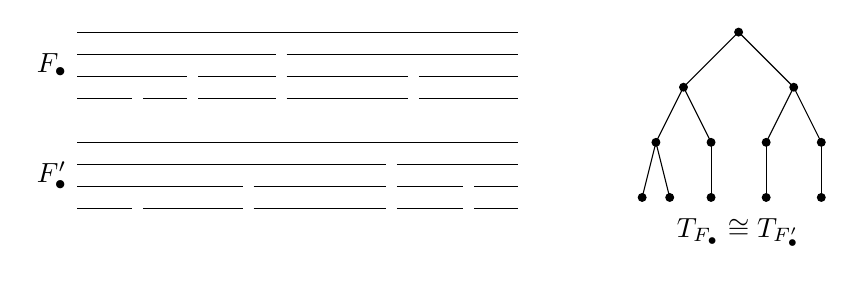
\begin{tikzpicture}[scale=1.4]
   %\draw [help lines] (0,0) grid (5,2);

   %filtration 1
        \draw [thin] (0,0) -- (4,0);
        
        \draw [thin] (0,-0.2) -- (1.8,-0.2); \draw [thin] (1.9,-0.2) -- (4,-0.2);
        
        \draw [thin] (0,-0.4) -- (1,-0.4); \draw [thin] (1.1,-0.4) -- (1.8,-0.4);
        \draw [thin] (1.9,-0.4) -- (3,-0.4); \draw [thin] (3.1,-0.4) -- (4,-0.4);
        
        \draw [thin] (0,-0.6) -- (0.5,-0.6); \draw [thin] (0.6,-0.6) -- (1,-0.6);
        \draw [thin] (1.1,-0.6) -- (1.8,-0.6);
        \draw [thin] (1.9,-0.6) -- (3,-0.6); \draw [thin] (3.1,-0.6) -- (4,-0.6);

        \draw (0,-0.3) node[left] {$\mc{F}_{\bullet}$};
        
        % filtration 2
        \draw [thin] (0,-1) -- (4,-1);
        
        \draw [thin] (0,-1.2) -- (2.8,-1.2); \draw [thin] (2.9,-1.2) -- (4,-1.2);
        
        \draw [thin] (0,-1.4) -- (1.5,-1.4); \draw [thin] (1.6,-1.4) -- (2.8,-1.4);
        \draw [thin] (2.9,-1.4) -- (3.5,-1.4); \draw [thin] (3.6,-1.4) -- (4,-1.4);
        
        \draw [thin] (0,-1.6) -- (0.5,-1.6); \draw [thin] (0.6,-1.6) -- (1.5,-1.6);
        \draw [thin] (1.6,-1.6) -- (2.8,-1.6);
        \draw [thin] (2.9,-1.6) -- (3.5,-1.6); \draw [thin] (3.6,-1.6) -- (4,-1.6);

        \draw (0,-1.3) node[left] {$\mc{F}'_{\bullet}$};
  
        % tree
        \draw[fill=black] (6,0) circle [radius = 1pt];
        
        \draw[fill=black] (5.5,-0.5) circle [radius = 1pt];
        \draw[thin] (6,0) -- (5.5,-0.5);
        \draw[fill=black] (6.5,-0.5) circle [radius = 1pt];
        \draw[thin] (6,0) -- (6.5,-0.5);

        \draw[fill=black] (5.25,-1) circle [radius = 1pt];
        \draw[thin] (5.5,-0.5) -- (5.25,-1);
        \draw[fill=black] (5.75,-1) circle [radius = 1pt];
        \draw[thin] (5.5,-0.5) -- (5.75,-1);
        
        \draw[fill=black] (6.25,-1) circle [radius = 1pt];
        \draw[thin] (6.5,-0.5) -- (6.25,-1);
        \draw[fill=black] (6.75,-1) circle [radius = 1pt];
        \draw[thin] (6.5,-0.5) -- (6.75,-1);

        \draw[fill=black] (5.125,-1.5) circle [radius = 1pt];
        \draw[thin] (5.25,-1) -- (5.125,-1.5);
        \draw[fill=black] (5.375,-1.5) circle [radius = 1pt];
        \draw[thin] (5.25,-1) -- (5.375,-1.5);
        
        \draw[fill=black] (5.75,-1.5) circle [radius = 1pt];
        \draw[thin] (5.75,-1) -- (5.75,-1.5);

        \draw[fill=black] (6.25,-1.5) circle [radius = 1pt];
        \draw[thin] (6.25,-1) -- (6.25,-1.5);
        \draw[fill=black] (6.75,-1.5) circle [radius = 1pt];
        \draw[thin] (6.75,-1) -- (6.75,-1.5);

        \draw (6,-1.6) node[below] {$T_{\mc{F}_{\bullet}} \cong T_{\mc{F}'_{\bullet}}$};

      \end{tikzpicture}
      \end{center}
\end{figure}

\begin{defn}
  Let $\mc{F}_{\bullet}$ and $\mc{F}_{\bullet}'$ be commonly indexed finite interval filtrations with associated tree $T$ and vertex-to-atom maps $\map{\alpha}{T}{\mc{F}_{N}}$ and $\map{\alpha'}{T}{\mc{F}_{N}'}$.
  For $\varepsilon \in (0,1)$, we say that $\mc{F}_{\bullet}$ and $\mc{F}_{\bullet}'$ are \emph{$\varepsilon$-close} if for all $v \in V(T)$,
  \begin{equation*}
    |\alpha(v) \Delta \alpha'(v)| = |(\alpha(v) \cup \alpha'(v)) \sm (\alpha(v) \cap \alpha'(v))| < \varepsilon,
  \end{equation*}
  and thus also
  \begin{equation*}
    |\alpha(v)| - |\alpha'(v)| < \varepsilon.
  \end{equation*}
\end{defn}

\begin{lem}\label{lem:closeness}
  Fix $N \in \N$ and let $(\mc{F}_{n})_{n=0}^{N}, (\mc{F}'_{n})_{n=0}^{N}$ be commonly indexed finite interval filtrations, with associated tree $T$ and vertex-to-atom maps $\map{\alpha}{T}{\mc{F}_{N}}$ and $\map{\alpha'}{T}{\mc{F}_{N}'}$.
  Then if $\mc{F}_{\bullet}$ and $\mc{F}_{\bullet}$ are $\varepsilon$-close, then for all $\mb{f} \in L^p(\mc{F}_{N};X)$ with $\|\mb{f}\|_{L^p(\mc{F}_{N};X)} = 1$,
  \begin{equation*}
    \sup_{0 \leq n \leq N} \|(\E^{\mc{F}_{n}} - \E^{\mc{F}_{n}'})\mb{f}\|_{L^p([0,1);X)} \lesssim_{\mc{F}_{\bullet}} \varepsilon^{1/p}.
  \end{equation*}
\end{lem}

\begin{proof}
  First write
  \begin{equation*}
    \|(\E^{\mc{F}_{n}} - \E^{\mc{F}_{n}'})\mb{f}\|_{L^p([0,1);X)} \leq \sum_{v \in V(T)} \Big\| \frac{\1_{\alpha(v)}}{|\alpha(v)|} \otimes \E(\mb{f}\1_{\alpha(v)}) - \frac{\1_{\alpha'(v)}}{|\alpha'(v)|} \otimes \E(\mb{f}\1_{\alpha'(v)}) \Big\|_{L^p([0,1);X)}.
  \end{equation*}
  By the $\varepsilon$-closeness condition, for all $v \in V(T)$ we have
  \begin{equation*}
    \begin{aligned}
      &\Big\| \frac{\1_{\alpha(v)}}{|\alpha(v)|} - \frac{\1_{\alpha'(v)}}{|\alpha'(v)|} \Big\|_{p} \\
      &= \frac{1}{|\alpha(v)|} \Big\| \1_{\alpha(v)} - \frac{|\alpha(v)|}{|\alpha'(v)|} \1_{\alpha'(v)} \Big\|_{p} \\
      &\leq \frac{1}{|\alpha(v)|} \Big( \| \1_{\alpha(v)} - \1_{\alpha'(v)} \|_{p} + \Big\| \Big( 1 - \frac{|\alpha(v)|}{|\alpha'(v)|} \Big) \1_{\alpha'(v)} \Big\|_{p} \Big) \\
      &\leq \frac{1}{|\alpha(v)|} \Big( \varepsilon^{1/p} + |\alpha'(v)|^{1/p}\Big(1 - \frac{|\alpha(v)|}{|\alpha'(v)|} \Big) \Big) \\
      &= \frac{1}{|\alpha(v)|} \Big( \varepsilon^{1/p} + |\alpha'(v)|^{\frac{1}{p} - 1} (|\alpha'(v)| - |\alpha(v)| ) \Big) \\
      &\leq \frac{1}{|\alpha(v)|} (\varepsilon^{1/p} + \varepsilon) 
      \lesssim_{\mc{F}_{\bullet}} \varepsilon^{1/p}.
  \end{aligned}
\end{equation*}
We also have
\begin{equation*}
  \begin{aligned}
    \big\| \E(\mb{f}\1_{\alpha(v)}) - \E(\mb{f}\1_{\alpha'(v)}) \big\|_{X}
    \leq \|\mb{f}\|_{L^\infty([0,1);X)} |\alpha(v) \Delta \alpha'(v)| \lesssim_{\mc{F}_{\bullet}} \varepsilon
  \end{aligned}
\end{equation*}
using that the $\sigma$-algebra $\mc{F}_{N}$ is finite to control $\|\mb{f}\|_{L^\infty([0,1);X)}$ by $\|\mb{f}\|_{L^p([0,1);X)} = 1$.
Thus for all $v \in V(T)$ we can estimate
\begin{equation*}
  \begin{aligned}
    &\Big\| \frac{\1_{\alpha(v)}}{|\alpha(v)|} \otimes \E(\mb{f}\1_{\alpha(v)}) - \frac{\1_{\alpha'(v)}}{|\alpha'(v)|} \otimes \E(\mb{f}\1_{\alpha'(v)}) \Big\|_{L^p([0,1);X)} \\
    &\leq \Big\| \Big( \frac{\1_{\alpha(v)}}{|\alpha(v)|} - \frac{\1_{\alpha'(v)}}{|\alpha'(v)|}\Big) \otimes \E(\mb{f}\1_{\alpha(v)}) \Big\|_{L^p([0,1);X)} \\
    &\qquad + \Big\| \frac{\1_{\alpha'(v)}}{|\alpha'(v)|} \otimes \big( \E(\mb{f}\1_{\alpha(v)}) -  \E(\mb{f}\1_{\alpha'(v)}) \big)\Big\|_{L^p([0,1);X)}\\
    &\leq  \Big\| \frac{\1_{\alpha(v)}}{|\alpha(v)|} - \frac{\1_{\alpha'(v)}} {|\alpha'(v)|} \Big\|_{p} \| \E(\mb{f}\1_{\alpha(v)}) \|_{X}
    + \Big\| \frac{\1_{\alpha'(v)}}{|\alpha'(v)|} \Big\|_{p} \big\|  \E(\mb{f}\1_{\alpha(v)}) -  \E(\mb{f}\1_{\alpha'(v)}) \big\|_{X} \\
    &\lesssim_{\mc{F}_{\bullet}} \varepsilon^{1/p} \|\mb{f}\|_{L^p([0,1);X)} + \varepsilon \lesssim \varepsilon^{1/p}.
  \end{aligned}
\end{equation*}
This completes the proof.
\end{proof}

% We say that a finite interval filtration $(\mc{F}_n)_{n=0}^{N}}$ is \emph{conditionally dyadic} if $\mc{F}_{N} \subset \mc{D}_{M}$ for some $M \in \N$: that is, if every atom in $\mc{F}_{N}$ can be written as a union of dyadic intervals $I$ of length $2^{-M}$ for some (potentially very large) $M$.
% Equivalently, all the conditional probabilities $|I|/|J|$, where $I$ is an atom of $\mc{F}_{n}$ and $J$ is an atom of $\mc{F}_{n+1}$, are of the form $2^{-j} k$ for some $j,k \in \N$.
% In the next lemma we show that finite interval filtrations can be approximated arbitrarily well by conditionally dyadic filtrations.

In the next lemma we show that finite interval filtrations can be approximated arbitrary well with filtrations that are very closely related to the dyadic filtration.

\begin{lem}\label{lem:dyadic-approximation}
  Let $(\mc{F}_{n})_{n=0}^{N}$ be a finite interval filtration and $\varepsilon \in (0,1)$.
  Then there is filtration $\mc{F}'_{\bullet}$ such that $\mc{F}_{\bullet}$ and $\mc{F}'_{\bullet}$ are commonly indexed and $\varepsilon$-close, with $\mc{F}'_{n} \subset \mc{D}_{m(n)}$ for some increasing sequence $m(0) < m(1) < \ldots < m(N)$, where $\mc{G}_{\bullet}$ is the dyadic filtration.
  Furthermore, for all $n \in \{0,1,\ldots,N\}$ we have
  \begin{equation}\label{eq:approx-CE-ident}
    \E^{\mc{F}'_{n}} = \E^{\mc{G}_{m(n)}} \E^{\mc{F}'_{N}}.
  \end{equation}
\end{lem}

\begin{proof}
  We construct $\mc{F}'_{\bullet}$ inductively, with the trivial base case $\mc{F}'_{0} = \mc{F}_{0} = \{\varnothing, [0,1)\}$.
  Having constructed $\mc{F}'_{n}$ as required, and with the sequence $m(0) < m(1) < \ldots < m(n)$ at hand, choose $m(n+1) > m(n)$ sufficiently large that each left endpoint $\ell(A)$, with $A$ an atom of $\mc{F}_{n+1}$, is within distance $\varepsilon/2$ of the set of dyadic numbers
  \begin{equation*}
    D_{m(n+1)} := \{2^{-m(n+1)}k : k \in \{0,1,\ldots,2^{m(n+1)} - 1\}\}.
  \end{equation*}
  For each atom $A$ of $\mc{F}_{n+1}$, choose a dyadic number $d_{A} \in D_{m(n+1)}$ with $|\ell(A) - d_{A}| < \varepsilon/2$.
  If $m(n+1)$ is sufficiently large we can ensure that the points $d_{A}$ are unique.
  Let $(d_{i})_{i=0}^{K}$ be the sequence of points $d_{A}$ in increasing order, and let
  \begin{equation*}
    \mc{F}'_{n+1} := \sigma([0,d_{0}), [d_{0}, d_{1}), \ldots, [d_{K},1)).
  \end{equation*}
  Note that $\mc{F}'_{n+1} \subset \mc{G}_{m(n+1)}$ by construction, and that
  \begin{equation*}
    |A \Delta [d_{A}, d_{A+1})| < \varepsilon
  \end{equation*}
  for all atoms $A \in \mc{F}_{n+1}$.
  Iterating this construction yields a filtration with the claimed properties, other than the conditional expectation identity \eqref{eq:approx-CE-ident} which remains to be shown.
  To show this, fix $\mb{f} \in L^1(\mc{F}_{N}')$ and $I \in \mc{F}_{n}'$: we will show that
  \begin{equation*}
    \int_{I} \E^{\mc{G}_{m(n)}} \E^{\mc{F}_{N}'} \mb{f} \, \dd t = \int_{I} \mb{f},
  \end{equation*}
  which establishes the identity via the defining property of conditional expectations.
  Since $I \in \mc{F}_{n}' \subset \mc{G}_{m(n)}$, $I$ can be written as a union of dyadic intervals $J \in \mc{D}_{m(n)}$, so
  \begin{equation*}
    \begin{aligned}
      \int_{I} \E^{\mc{G}_{m(n)}} \E^{\mc{F}_{N}'} \mb{f}(t) \, \dd t
      &= \sum_{\substack{J \in \mc{D}_{m(n)} \\ J \subset I}} \int_{J} \E^{\mc{G}_{m(n)}} \E^{\mc{F}_{N}'} \mb{f}(t) \, \dd t \\
      &= \sum_{\substack{J \in \mc{D}_{m(n)} \\ J \subset I}} \int_{J} \E^{\mc{F}_{N}'} \mb{f}(t) \, \dd t
      = \int_{I} \E^{\mc{F}_{N}'} \mb{f}(t) \, \dd t = \int_{I} \mb{f}(t) \, \dd t
    \end{aligned}
  \end{equation*}
  using $J \in \mc{G}_{m(n)}$ and $I \in \mc{F}_{n}' \subset \mc{F}_{N}'$.
\end{proof}

\begin{thm}\label{thm:dyadic-UMD}
  Suppose that $p \in (1,\infty)$ and that $X$ has the dyadic UMD property.
  Then $X$ is UMD.
\end{thm}

\begin{proof}
  By Proposition \ref{prop:UMD-FIF} it suffices to consider martingales $\mb{f}_{\bullet}$ on $[0,1)$ with respect to finite interval filtrations $(\mc{F}_{n})_{n=0}^{N}$.
  By homogeneity we may assume that $\|\mb{f}_{N}\|_{L^p([0,1);X)} = 1$.
  Let $(\xi_{n})_{n=0}^{N}$ be a sequence of signs.
  Fix $\varepsilon \in (0,1)$ and let $\mc{F}'_{\bullet}$ be a filtration as in Lemma \ref{lem:dyadic-approximation}, such that $\mc{F}_{n}' \subset \mc{D}_{m(n)}$ for all $n$ and such that $\mc{F}_{\bullet}$ and $\mc{F}_{\bullet}'$ are commonly indexed and $\varepsilon$-close.
  Let $\mb{f}_{\bullet}$ be a martingale with respect to a finite interval filtration $\mc{F}_{\bullet}$, and let $\mc{F}'_{\bullet}$ be an $\varepsilon$-close filtration as in the previous lemma.
  Then we have
  \begin{equation*}
    \begin{aligned}
      &\Big\| \sum_{n=0}^{N} \xi_{n} (\E^{\mc{F}_{n}} - \E^{\mc{F}_{n-1}}) \mb{f}_{N} \Big\|_{L^p([0,1);X)} \\
      &= \Big\| \sum_{n=0}^{N} \xi_{n} (\E^{\mc{F}'_{n}} - \E^{\mc{F}'_{n-1}}) \mb{f}_{N} \Big\|_{L^p([0,1);X)} \\
      &+ \sum_{n=0}^{N} \Big( \| (\E^{\mc{F}_{n}} - \E^{\mc{F}'_{n}}) \mb{f}_{N}\|_{L^p([0,1);X)}
      +  \| (\E^{\mc{F}'_{n}} - \E^{\mc{F}'_{n-1}}) \mb{f}_{N} \|_{L^p([0,1);X)} \Big).
    \end{aligned}
  \end{equation*}
  By $\varepsilon$-closeness, the second term is bounded by $C_{\mc{F}_{\bullet}} N \varepsilon^{1/p}$ (Lemma \ref{lem:closeness}, here we use $\|\mb{f}_{N}\|_{L^p([0,1);X)} = 1$).
  To control the first term we write
  \begin{equation*}
    \Big\| \sum_{n=0}^{N} \xi_{n} (\E^{\mc{F}'_{n}} - \E^{\mc{F}'_{n-1}}) \mb{f}_{N} \Big\|_{L^p([0,1);X)}
    = \Big\| \sum_{n=0}^{N} \xi_{n} (\E^{\mc{G}_{m(n)}} - \E^{\mc{G}_{m(n-1)}}) \E^{\mc{F}'_{N}} \mb{f}_{N} \Big\|_{L^p([0,1);X)}
  \end{equation*}
  using the identity \eqref{eq:approx-CE-ident}.
  By a telescoping sum argument we have
  \begin{equation*}
    \begin{aligned}
      &\Big\| \sum_{n=0}^{N} \xi_{n} (\E^{\mc{G}_{m(n)}} - \E^{\mc{G}_{m(n-1)}}) \E^{\mc{F}'_{N}} \mb{f}_{N} \Big\|_{L^p([0,1);X)} \\
      &\qquad = \Big\| \sum_{m=0}^{m(N)} \tilde{\xi}_{m} (\E^{\mc{G}_{m}} - \E^{\mc{G}_{m-1}}) \E^{\mc{F}'_{N}} \mb{f}_{N} \Big\|_{L^p([0,1);X)}
    \end{aligned}
  \end{equation*}
  for some sequence $\tilde{\xi}_{\bullet}$.
  Thus the assumed UMD property with respect to the dyadic filtration yields
  \begin{equation*}
    \begin{aligned}
      \Big\| \sum_{n=0}^{N} \xi_{n} (\E^{\mc{G}_{m(n)}} - \E^{\mc{G}_{m(n-1)}}) \E^{\mc{F}'_{N}} \mb{f}_{N} \Big\|_{L^p([0,1);X)}
      &\leq C \|\E^{\mc{F}'_{N}} \mb{f}_{N}\|_{L^p([0,1);X)} \\
      &\leq C\|\mb{f}_{N}\|_{L^p([0,1);X)}.
    \end{aligned}
    \end{equation*}
    All up we have
    \begin{equation*}
      \Big\| \sum_{n=0}^{N} \xi_{n} d\mb{f}_{N} \Big\|_{L^p([0,1);X)} \leq C\|\mb{f}_{N}\|_{L^p([0,1);X)} + C_{\mc{F}_{\bullet}} N \varepsilon^{1/p},
    \end{equation*}
    and since $\varepsilon \in (0,1)$ was arbitrary this completes the proof.
  \end{proof}

  For future reference we provide a useful characterisation of martingales on the dyadic filtration.

  \begin{prop}\label{prop:PW-martingales}
    Let $X$ be a Banach space and $\mb{f}_{\bullet}$ an $X$-valued martingale on $[0,1)$ with respect to the dyadic filtration $\mc{F}_{\bullet}$.
    Then there exist functions $\mb{\phi}_{n} \colon \{-1,1\}^{n-1} \to X$ ($\mb{\phi}_{1}$ is simply a constant in $X$) such that
    \begin{equation*}
      d\mb{f}_{n}(t) = r_{n}(t) \mb{\phi}_{n}(r_1(t), r_{2}(t)\ldots, r_{n-1}(t)) \qquad \forall n \geq 1,
    \end{equation*}
    where $(r_{n})_{n \geq 1}$ are the Rademacher functions defined on $[0,1)$, i.e.
    \begin{equation*}
      r_{n} := \sgn(\sin(2^n \pi t))
    \end{equation*}
    (see Example \ref{eg:analyst-rademachers}).
  \end{prop}

  \begin{proof}
    Write
    \begin{equation*}
      d\mb{f}_{n} = \sum_{I \in \mc{D}_{n-1}} (\1_{I_+} + \1_{I_{-}}) d\mb{f}_{n}
    \end{equation*}
    where $I_-$ and $I_+$ are the left and right halves of the interval $I$.
    Since $d\mb{f}_{n}$ is $\mc{F}_{n}$-measurable, it is constant on the intervals $I_\pm$ for $I \in \mc{D}_{n-1}$: let $\mb{x}_{I}$ denote the value of $d\mb{f}_{n}$ on $I_+$.
    Since $\E^{\mc{F}_{n-1}}d\mb{f}_{n} = 0$, we must have that $d\mb{f}_{n} = -\mb{x}_{I}$ on $I_{-}$, and so
    \begin{equation*}
      d\mb{f}_{n} = \sum_{I \in \mc{D}_{n-1}} (\1_{I_+} - \1_{I_{-}}) \otimes \mb{x}_{I} = r_{n} \tilde{\mb{\phi}}, \qquad \tilde{\mb{\phi}} := \sum_{I \in \mc{D}_{n-1}} \1_{I} \otimes \mb{x}_{I}.
    \end{equation*}
    The function $\tilde{\mb{\phi}} \colon [0,1) \to X$ is $\mc{F}_{n-1}$-measurable, and the $\sigma$-algebras $\mc{F}_{n-1}$ and $\sigma(r_{1}, r_{2}, \ldots, r_{n-1})$ are both generated by $2^{n-1}$ atoms, so we have that
    \begin{equation*}
      \tilde{\mb{\phi}} = \mb{\phi}(r_{1}, r_{2}, \ldots, r_{n-1})
    \end{equation*}
    for some $\mb{\phi} \in \{-1,1\}^{n-1} \to X$.
  \end{proof}

  One last observation.
  Let $\map{\varepsilon}{[0,1)}{\{-1,+1\}}$ be an arbitrary Rademacher variable on the unit interval (one could take $\varepsilon = r_{1}$ as a concrete example), and consider the finite Rademacher sequence $(\varepsilon_{n})_{n = 1}^N$ on $[0,1)^{N}$ defined by
  \begin{equation*}
    \varepsilon_{n}(\omega) := \varepsilon(\omega_{n}) \qquad \forall \omega \in [0,1)^{N}.
  \end{equation*}
  Then given an $X$-valued martingale $\mb{f}_{\bullet}$ with respect to the dyadic filtration on $[0,1)$, by Proposition \ref{prop:PW-martingales} and a change of variables there exist functions $\mb{\phi}_{n} \colon \{-1,1\}^{n-1} \to X$ such that
  \begin{equation*}
    \begin{aligned}
      \Big\| \sum_{n=1}^{N} \xi_{n}  d\mb{f}_{n}(t) \Big\|_{L^p([0,1);X)}
      &= \Big\| \sum_{n=1}^{N} \xi_{n} r_{n} \mb{\phi}_{n}(r_{1}, r_{2}, \ldots, r_{n-1}) \Big\|_{L^p([0,1);X)} \\
      &= \Big\| \sum_{n=1}^{N} \xi_{n} \varepsilon_{n} \mb{\phi}_{n}(\varepsilon_{1}, \varepsilon_{2}, \ldots, \varepsilon_{n-1}) \Big\|_{L^p([0,1)^{N};X)}
    \end{aligned}
  \end{equation*}
  for any sequence of signs $\xi_{\bullet}$.
  Note also that for all $n \in \{1,2,\ldots,N\}$, the functions
  \begin{equation*}
    \varepsilon_{n} \mb{\phi}_{n}(\varepsilon_{1}, \varepsilon_{2}, \ldots, \varepsilon_{n-1}) \colon [0,1)^{N} \to X
  \end{equation*}
  have vanishing integral, as
  \begin{equation*}
    \begin{aligned}
      &\int_{[0,1)^{N}} \varepsilon_{n}(\omega) \mb{\phi}_{n}(\varepsilon_{1}(\omega), \varepsilon_{2}(\omega), \ldots, \varepsilon_{n-1}(\omega)) \, \dd \omega \\
    &= \Big( \int_{[0,1)} \varepsilon(\omega_{n}) \, \dd\omega_{n} \Big) \int_{[0,1)^{N-1}} \mb{\phi}_{n}(\varepsilon_{1}(\omega), \varepsilon_{2}(\omega), \ldots, \varepsilon_{n-1}(\omega)) \, \dd \omega = \mb{0}.
  \end{aligned}
\end{equation*}
We will use these observations shortly.
  
  \section{The Hilbert transform on the torus}

  To prove the UMD property from boundedness of the Hilbert transform, we will make one further reduction: we will first deduce the boundedness of the \emph{Hilbert transform on the ($1$-dimensional) torus}.
  The $1$-dimensional `torus', known to more reasonable  mathematicians as the `circle', is the abelian group
  \begin{equation*}
    \T = [0,1) \cong \R / \Z
  \end{equation*}
  with addition $+$ given by the usual addition on $\R$, modulo $\Z$.
  We equip $\T$ with the Lebesgue measure, and of course this measure is translation invariant with respect to addition.
  Naturally every function on the torus can be identified with a $1$-periodic function on $\R$, and conversely.
  We consider more generally the $N$-dimensional torus
  \begin{equation*}
    \T^{N} = [0,1)^{N} \cong \R^{N} / \Z^{N}, 
  \end{equation*}
  and the aforementioned properties of $\T$ also hold for $\T^{N}$.

  Fix a dimension $N \in \N$.
  For a complex Banach space $X$ and $\mb{f} \in L^1(\T^{N};X)$ we define the Fourier transform $\map{\hat{\mb{f}}}{\Z^{N}}{X}$ by
  \begin{equation*}
    \hat{\mb{f}}(n) := \int_{\T^{N}} e^{2\pi i t \cdot n} \mb{f}(t) \, \dd t \qquad \forall n = (n_1,\ldots,n_N) \in \Z^{N}.
  \end{equation*}
  Note that $\mb{f}$ has vanishing integral if and only if $\hat{\mb{f}}(0) = \mb{0}$.
  A function $\mb{f} \in L^1(\T^{N};X)$ is called a \emph{trigonometric polynomial} if $\hat{\mb{f}}$ is finitely supported, and in this case we have the finite sum
  \begin{equation}\label{eq:trigpoly}
    \mb{f}(t) = \sum_{n \in \Z^{N}} e^{2\pi i t \cdot n} \hat{\mb{f}}(n) = \sum_{n \in \Z^{N}} e_{n}(t) \hat{\mb{f}}(n),
  \end{equation}
  writing $e_{n}(t) := e^{2\pi i t \cdot n}$ for all $t \in \T^{N}$.
  In the scalar-valued setting, the trigonometric polynomials are dense in $L^p(\T^{N})$ for all $p \in [1,\infty]$, and thus for all $X$ the trigonometric polynomials are dense in $L^p(\T^{N};X)$ for all $p \in [1,\infty)$.

  By analogy with the Fourier multiplier representation of the Hilbert transform on the real line, we define the Hilbert transform on the $1$-dimensional torus, initially just on trigonomeric polynomials.
  \begin{defn}
    Let $X$ be a complex Banach space and $\mb{f} \in L^1(\T;X)$ a trigonometric polynomial.
    Then we define the Hilbert transform $H_{\T}\mb{f}$ by
    \begin{equation*}
      H_{\T} \mb{f} := -i \sum_{n \in \Z} \sgn(n) e_{n} \otimes \hat{\mb{f}}(n) = -i \Big( \sum_{n > 0} - \sum_{n < 0} \Big) e_{n} \otimes \hat{\mb{f}}(n).
    \end{equation*}  
  \end{defn}

  The boundedness of $H_{\T}$ on $L^p(\T;X)$ can be deduced from boundedness of the Hilbert transform $H$ on $L^p(\R;X)$.
  The argument below is adapted to the Hilbert transform, but a more general `transference' result can be proven for general Fourier multipliers, including those with operator-valued symbols (see \cite[\textsection 5.7]{HNVW16}).
  First we show how to relate the $L^p$-norm of a function on $\T$ with that of (localisations of) its periodic extension.

  \begin{lem}\label{lem:transference}
    Let $X$ be a Banach space, $p \in [1,\infty)$, $\mb{f} \in L^p(\T;X)$, and let $\phi \in \Sch(\R)$ be a scalar-valued Schwartz function on the real line.
    For all $\lambda > 0$, let $\Dil_{\varepsilon}^{p} \phi$ be the $L^p$-normalised dilation of $\mb{f}$ by $\lambda$: that is, for $t \in \R$, $(\Dil_{\lambda}^{p}\phi)(t) := \lambda^{-1/p} \phi(t/\lambda)$.
    Then
    \begin{equation*}
        \lim_{\lambda \to \infty} \| (\Dil_{\lambda}\phi) \mb{f} \|_{L^p(\R;X)} = \|\mb{f}\|_{L^p(\T;X)}\|\phi\|_{L^p(\R)}.
    \end{equation*}
  \end{lem}

  \begin{proof}
    The left hand side, to the power $p$, can be written as
    \begin{equation}\label{eq:bracketed-quantity}
      \lim_{\lambda \to \infty} \int_{\R} \lambda^{-1}|\phi(t/\lambda)|^{p} \|\mb{f}(t)\|_{X}^{p} \, \dd t
      = \lim_{\lambda \to \infty} \int_{0}^{1} \|\mb{f}(t)\|_{X}^{p} \Big( \sum_{k \in \Z} \frac{|\phi((t+k)/\lambda)|^{p}}{\lambda} \Big) \, \dd t.
  \end{equation}
  For all $t \in (0,1)$ and $\lambda > 1$, since $\phi \in \Sch(\R)$, there exists $C < \infty$ such that
  \begin{equation*}
    \begin{aligned}
      \sum_{k \in \Z} \frac{|\phi((t+k)/\lambda)|^{p}}{\lambda}
      &\leq \frac{C}{\lambda} \sum_{k \in \Z} \min(1,|t+k|/\lambda)^{-2p} \\
      &\leq \frac{C}{\lambda} \Big( \sum_{|k| \leq 2\lambda} 1 + \sum_{|k| > 2\lambda}  (|t+k|/\lambda)^{-2p} \Big) \\
      &\lesssim \frac{1}{\lambda} \Big( \lambda + \lambda^{2p} \sum_{k > 2\lambda} k^{-2p} \Big) \\
      &\leq 1 + \lambda^{2p-1} \int_{2\lambda}^\infty t^{-2p} \, \dd t \Big) \\
      &\simeq 1 + \lambda^{2p-1} \lambda^{-2p+1} \simeq 1
    \end{aligned}
  \end{equation*}
  using that $2p > 1$.
  Thus the bracketed quantity in \eqref{eq:bracketed-quantity} is bounded uniformly in $t$ as $\lambda \to \infty$, and we can use dominated convergence to write
  \begin{equation*}
    \begin{aligned}
      &\lim_{\lambda \to \infty} \int_{0}^{1} \|\mb{f}(t)\|_{X}^{p} \Big( \sum_{k \in \Z} \frac{|\phi((t+k)/\lambda)|^{p}}{\lambda} \Big) \, \dd t \\
      &= \int_{0}^{1} \|\mb{f}(t)\|_{X}^{p} \lim_{\lambda \to \infty} \Big( \sum_{k \in \Z} \frac{|\phi((t+k)/\lambda)|^{p}}{\lambda} \Big) \, \dd t \\
      &= \int_{0}^{1} \|\mb{f}(t)\|_{X}^{p} \Big( \int_{\R} |\phi(s)|^{p} \, \dd s\Big) \, \dd t
    \end{aligned}
  \end{equation*}
  since the bracketed quantity is a Riemann sum.
  The result follows.
  \end{proof}

  \begin{prop}\label{prop:UMD-HTT}
    Let $X$ be a complex Banach space and $p \in (1,\infty)$.
    Suppose that the Hilbert transform $H \in \Lin(L^p(\R))$ admits a bounded $X$-valued extension.
    Then for all trigonometric polynomials $\mb{f} \in L^1(\T;X)$, we have
    \begin{equation*}
      \|H_{\T} \mb{f}\|_{L^p(\T;X)} \lesssim_{p,X} \|\mb{f}\|_{L^p(\T;X)}.
    \end{equation*}
  \end{prop}
  
  \begin{proof}
    First write
    \begin{equation*}
      \begin{aligned}
        H_{\T} \mb{f}
        &= \sum_{n \in \Z} -i \sgn(n) e_{n} \otimes \hat{\mb{f}}(n) \\
        &= \frac{1}{2} \Big(
        \sum_{n \in \Z} -i \sgn\Big(n+\frac{1}{2}\Big) e_{n} \otimes \hat{\mb{f}}(n)
        + \sum_{n \in \Z} -i \sgn\Big(n-\frac{1}{2}\Big) e_{n} \otimes \hat{\mb{f}}(n) \Big),
      \end{aligned}
    \end{equation*}
    noting that $\sgn(n) = \sgn(n \pm \frac{1}{2})$ for all $n \neq 0$, and that $\sgn(1/2) = -\sgn(-1/2)$.
    Thus it suffices to prove the estimates
    \begin{equation*}
      \Big\| \sum_{n \in \Z} -i \sgn\Big(n\pm\frac{1}{2}\Big) e_{n} \otimes \hat{\mb{f}}(n) \Big\|_{L^p(\T;X)} \lesssim_{p,X} \|\mb{f}\|_{L^p(\T;X)}
    \end{equation*}
    for both choices of sign $\pm$.
    Since the argument is identical for both choices, we just take $+$.
    
    Fix a Schwartz function $\phi \in \Sch(\R)$ such that the Fourier transform $\hat{\phi}$ is supported in $(-1/2,1/2)$, and normalise such that $\|\phi\|_{p} = 1$.
    Fix $\lambda > 1$, and note that $\Dil^{p}_{\lambda}\phi$ is also supported in $(-1/2,1/2)$, with $\|\Dil^{p}_{\lambda}\phi\|_{p} = 1$.
    We will use that $H \otimes I$ has a bounded extension to $L^p(\R;X)$, where $H$ is the scalar-valued Hilbert transform (Theorem \ref{thm:Burkholder}).
    Observe that
    \begin{equation*}
      \begin{aligned}
        (H \otimes I)((\Dil_{\lambda}^{p} \phi) e_{\frac{1}{2}} \mb{f})
        &= (H \otimes I)\Big( \sum_{n \in \Z} (\Dil_{\lambda}^{p} \phi) e_{n + \frac{1}{2}} \otimes \hat{\mb{f}}(n) \Big) \\
        &= \sum_{n \in \Z} H((\Dil_{\lambda}^{p}\phi) e_{n + \frac{1}{2}}) \otimes \hat{\mb{f}}(n)
      \end{aligned}
    \end{equation*}
    since the sum has finitely many nonzero terms.
    For each $n \in \Z$, the modulation $(\Dil_{\lambda}^{p}\phi) e_{n + \frac{1}{2}} = \Mod_{n + \frac{1}{2}} (\Dil_{\lambda}^{p}\phi)$ has Fourier transform supported in $(n, n+1)$, so
    \begin{equation*}
          H((\Dil_{\lambda}^{p}\phi) e_{n + \frac{1}{2}}) = -i\sgn(n) (\Dil_{\lambda}^{p}\phi) e_{n + \frac{1}{2}} = -i\sgn\big(n+\frac{1}{2}\big) (\Dil_{\lambda}^{p}\phi) e_{n} e_{\frac{1}{2}}
    \end{equation*}
    which lets us write
    \begin{equation*}
       (H \otimes I)((\Dil_{\lambda}^{p}\phi) e_{\frac{1}{2}} \mb{f}) = (\Dil_{\lambda}^{p}\phi) e_{\frac{1}{2}} \sum_{n \in \Z} -i\sgn\big(n + \frac{1}{2}\big)  e_{n} \otimes \hat{\mb{f}}(n)
     \end{equation*}
     Now we use Lemma \ref{lem:transference} backwards, invoke boundedness of $H \otimes I$ on $L^p(\R;X)$, and then use Lemma \ref{lem:transference} forwards:
     \begin{equation*}
       \begin{aligned}
         &\Big\| \sum_{n \in \Z} -i \sgn\Big(n\pm\frac{1}{2}\Big) e_{n} \otimes \hat{\mb{f}}(n) \Big\|_{L^p(\T;X)} \\
         &= \Big\| e_{\frac{1}{2}} \sum_{n \in \Z} -i \sgn\Big(n\pm\frac{1}{2}\Big) e_{n} \otimes \hat{\mb{f}}(n) \Big\|_{L^p(\T;X)} \\
         &= \Big\| e_{\frac{1}{2}} \sum_{n \in \Z} -i \sgn\Big(n\pm\frac{1}{2}\Big) e_{n} \otimes \hat{\mb{f}}(n) \Big\|_{L^p(\T;X)} \|\phi\|_{L^p(\R)} \\
         &= \lim_{\lambda \to \infty} \Big\| (\Dil_{\lambda}^{p}\phi) e_{\frac{1}{2}} \sum_{n \in \Z} -i \sgn\Big(n\pm\frac{1}{2}\Big) e_{n} \otimes \hat{\mb{f}}(n) \Big\|_{L^p(\R;X)} \\
         &= \lim_{\lambda \to \infty} \big\| (H \otimes I)((\Dil_{\lambda}^{p} \phi)e_{\frac{1}{2}} \mb{f}) \big\|_{L^p(\R;X)} \\
         &\lesssim_{p,X} \lim_{\lambda \to \infty} \big\| e_{\frac{1}{2}} (\Dil_{\lambda}^{p} \phi)  \mb{f} \big\|_{L^p(\R;X)} 
         = \lim_{\lambda \to \infty} \big\| (\Dil_{\lambda}^{p} \phi)  \mb{f} \big\|_{L^p(\R;X)} 
         = \| \mb{f} \|_{L^p(\T;X)}.
       \end{aligned}
     \end{equation*}
     The same argument with $k - \frac{1}{2}$ in place of $k + \frac{1}{2}$ completes the proof.
  \end{proof}

  In the argument used to deduce the UMD property from boundedness of the Hilbert transform, we use not only the boundedness of $H_{\T}$, but also of associated operators on $\T^{N}$.

  \begin{defn}\label{defn:higher-HT}
    Let $X$ be a complex Banach space such that $H_{\T}$ is bounded on $L^p(\T;X)$, and fix $N \in \N$.
    For $n \leq N$, let $\T_{n}$ denote the $n$th copy of $\T$ in the product space $\T^{N}$, so that $\T^{N} = \T_{1} \times \cdots \times \T_{N}$.
    Let $H_{\T,n}$ be the bounded linear operator on $L^p(\T^{N};X)$ which acts as $H_{\T}$ on $\T_{n}$, and as the identity operator in all other coordinates.\footnote{This operator can be written as $H_{\T,n} = I \otimes \cdots \otimes I \otimes H_{\T} \otimes I \otimes \cdots \otimes I$.}
    That is, for $\mb{f} \in L^p(\T^{N};X)$, we have
    \begin{equation*}
      H_{\T,n}\mb{f}(t_{1}, \ldots, t_{N}) = (H_{\T} \mb{f}(t_{1}, \ldots, t_{n-1}, \bullet, t_{n+1}, \ldots, t_{N}))(t_{n})
    \end{equation*}
    Where the functions $\mb{f}(t_{1}, \ldots, t_{n-1}, \bullet, t_{n+1}, \ldots, t_{N}) \colon \T \to X$ are given by
    \begin{equation*}
      \mb{f}(t_{1}, \ldots, t_{n-1}, \bullet, t_{n+1}, \ldots, t_{N})(s) := \mb{f}(t_{1}, \ldots, t_{n-1}, s, t_{n+1}, \ldots, t_{N})
    \end{equation*}
    By Fubini's theorem, these definitions make sense almost everywhere, and the operators $H_{\T,n}$ are bounded on $L^p(\T^{N};X)$ for all $N \geq n$, with norms bounded uniformly in $N$ and $n$.
  \end{defn}

  In the following section we will freely identify functions $\mb{f} \in L^p(\T^{N};X)$ with functions $\mb{f} \in L^p(\T ; L^p(\T^{N-1};X))$ when $p \in (1,\infty)$: Fubini's theorem justifies this.


\section{Bourgain's theorem: from the Hilbert transform to UMD}

In this section we prove Theorem \ref{thm:Bourgain}: if the Banach space $X$ is such that the Hilbert transform $H \in \Lin(L^p(\R))$ admits a bounded $X$-valued extension for some $p \in (1,\infty)$, then $X$ is UMD.
By Theorem \ref{thm:dyadic-UMD} it suffices to show that $X$ has the dyadic $\UMD_{p}$ property.
Furthermore, by Proposition \ref{prop:UMD-HTT} we know that the Hilbert transform $H_{\T}$ on the torus is bounded on $L^p(\T;X)$, and thus so are the operators $H_{\T,n}$ on $L^p(\T^{N};X)$ from Definition \ref{defn:higher-HT}.
Given a Banach space $Y$ we will write
\begin{equation*}
  L^p_{0}(\T;Y) := \Big\{\mb{f} \in L^p(\T;Y) : \int_{\T} \mb{f} = \mb{0} \Big\}
\end{equation*}
to denote the subspace of functions with vanishing integral.

The key estimate is the following, whose proof we will briefly defer.
\begin{prop}\label{prop:Bourgain-H}
  Let $p \in (1,\infty)$, and suppose $X$ is a complex Banach space such that $H_{\T}$ is bounded on $L^p(\T;X)$.
  Then for all finite sign sequences $(\xi_{n})_{n=1}^{N}$ and all functions $\mb{f}_{n} \in L^p_{0}(\T_{n};L^p(\T^{n-1};X))$ with $1 \leq n \leq N$, under the natural identification $L^p(\T^{n};X) \subset L^p(\T^{N};X)$, we have
  \begin{equation*}
    \Big\| \sum_{n=1}^{N} \xi_{k} H_{\T,n} \mb{f}_{n} \Big\|_{L^p(\T^{N};X)} \lesssim_{p,X} \Big\| \sum_{n=1}^{N} \mb{f}_{n} \Big\|_{L^p(\T^{N};X)}.
  \end{equation*}
\end{prop}

Assuming this for the moment, let's prove Bourgain's theorem.
\begin{proof}[Proof of Theorem \ref{thm:Bourgain}, assuming Proposition \ref{prop:Bourgain-H}]
  It suffices to consider finite $X$-valued martingales $(\mb{f}_n)_{n=0}^{N}$ on $[0,1)$ with respect to the dyadic filtration, and without loss of generality we can assume $\mb{f}_{0} \equiv \mb{0}$.
  By Proposition \ref{prop:PW-martingales} and the remark following its proof, there exist functions $\map{\mb{\phi}_{n}}{\{-1,1\}^{n-1}}{X}$ such that we are reduced to proving
  \begin{equation*}
    \Big\| \sum_{n=1}^{N} \xi_{n} \varepsilon_{n} \mb{\phi}_{n}(\varepsilon_{1}, \varepsilon_{2}, \ldots, \varepsilon_{n-1}) \Big\|_{L^p([0,1)^{N};X)} \lesssim \Big\| \sum_{n=1}^{N} \varepsilon_{n} \mb{\phi}_{n}(\varepsilon_{1}, \varepsilon_{2}, \ldots, \varepsilon_{n-1}) \Big\|_{L^p([0,1)^{N};X)}
  \end{equation*}
  where $(\varepsilon_{n})_{n=1}^{N}$ is a Rademacher sequence on $[0,1)^{N}$ with each $\varepsilon_{n}$ depending only on the $n$-th coordinate.
  Thus it suffices to show
  \begin{equation*}
    \Big\| \sum_{n=1}^{N} \xi_{n} \mb{g}_{n} \Big\|_{L^p(\T^{N};X)} \lesssim \Big\| \sum_{n=1}^{N} \mb{g}_{n} \Big\|_{L^p(\T^{N};X)}
  \end{equation*}
  for all $\mb{g}_{n} \in L_{0}^p(\T_{n};L^{p}(\T^{n-1};X)) \subset L^p(\T^{N};X)$.
  The Hilbert transform $H \in \Lin(L^p(\R))$ having a bounded $X$-valued extension implies that $H_{\T}$ is bounded on $L^p(\T;X)$ (Lemma \ref{lem:transference}), so using that $H_{\T,n}^{2} = -I$ on $L^p(\T^{N};X)$ for all $n \leq N$, we can use Proposition \ref{prop:Bourgain-H} twice to estimate
  \begin{equation*}
    \begin{aligned}
      \Big\| \sum_{n=1}^{N} \xi_{n} \mb{g}_{n} \Big\|_{L^p(\T^{N};X)}
      &= \Big\| \sum_{n=1}^{N} \xi_{n} H_{\T,n} (H_{\T,n} \mb{g}_{n}) \Big\|_{L^p(\T^{N};X)} \\
      &\lesssim_{p,X}  \Big\| \sum_{n=1}^{N} H_{\T,n} \mb{g}_{n} \Big\|_{L^p(\T^{N};X)} 
      \lesssim_{p,X}  \Big\| \sum_{n=1}^{N} \mb{g}_{n} \Big\|_{L^p(\T^{N};X)},
    \end{aligned}
  \end{equation*}
  completing the proof.
\end{proof}

So we are left with proving Proposition \ref{prop:Bourgain-H}.
This relies on a clever choice of isometry of $L^p(\T^{N};X)$ into $L^p(\T; L^p(\T^{N};X))$, which intertwines the operators $H_{\T,n}$ with the $L^p(\T^{N};X)$-valued Hilbert transform $\tilde{H}_{\T}$ in a special way.

\begin{lem}\label{lem:Bourgain}
  Fix a sequence $M_{\bullet} = (M_{n})_{n=1}^{N}$ of nonzero integers, and define $\mc{B}_{M} \colon L^p(\T^{N};X) \to L^{p}(\T; L^p(\T^{N};X))$ by
  \begin{equation*}
    (\mc{B}_{M} \mb{g}(s))(t_{1}, \ldots, t_{N}) := \mb{g}(t_{1} + M_{1} s, \ldots, t_{N} + M_{N} s).
  \end{equation*}
  Then $\mc{B}_{M}$ is an isometry which maps trigonometric polynomials into trigonometric polynomials.
  Furthermore, given a sequence of trigonometric polynomials
  \begin{equation*}
    \mb{f}_{n} \in L^p_{0}(T_{n}; L^p(\T^{n-1};X))
  \end{equation*}
  (note the vanishing integral condition), if the sequence $|M_{1}|, |M_{2}|, \ldots, |M_{N}|$ is sufficiently rapidly increasing, we have
  \begin{equation}\label{eq:B-ident}
    \tilde{H}_{\T} (\mc{B}_{M} \mb{f}_{n}) = \sgn(M_{n}) \mc{B}_{M} H_{\T,n} \mb{f}_{n}
  \end{equation}
  where $\tilde{H}_{\T}$ is the Hilbert transform on $L^p(\T; L^p(\T^{N};X))$.
\end{lem}

\begin{proof}
  That $\mc{B}_{M}$ is an isometry follows from translation invariance of the measure on $\T$: for all $\mb{g} \in L^p(\T^{N};X)$, by Fubini's theorem,
  \begin{equation*}
    \begin{aligned}
      \|\mc{B}_{M} \mb{g} \|_{L^p(\T;L^p(\T^{N};X))}^{p}
      &=\int_{\T} \int_{\T^{N}} \|\mb{g}(t_{1} + M_{1} s, \ldots, t_{N} + M_{N} s )\|_{X}^{p} \, \dd t_{1} \, \cdots \dd t_{N} \, \dd s \\
      &= \int_{\T} \int_{\T^{N}} \|\mb{g}(t_{1}, t_{2} + M_{2} s, \ldots t_{N} + M_{N} s )\|_{X}^{p} \, \dd t_{1} \, \cdots \dd t_{N} \, \dd s \\
      &= \cdots \\
      &= \int_{\T} \|\mb{g}\|_{L^p(\T^{n};X)}^{p} \, \dd s = \|\mb{g}\|_{L^p(\T^{n};X)}^{p}.
    \end{aligned}
  \end{equation*}
  That $\mc{B}_{M}$ maps trigonometric polynomials to trigonometric polynomials is Exercise \ref{ex:B-trigpoly}.
  
  Now consider $\mb{f}_{n} \in L^{p}_{0}(\T_{n} ; L^p(\T^{n-1};X))$ for $n \in \{1,2,\ldots,N\}$.
  Viewing $\mb{f}_{n}$ as a function on $\T^{n}$, for $t \in \T^{n}$ write
  \begin{equation*}
    \begin{aligned}
      \mb{f}_{n}(t)
      &= \sum_{\substack{m \in \Z^{n} \\ m_{n} \neq 0}} e_{m}(t) \hat{\mb{f}_{n}}(m)  \\
      &= \sum_{\substack{m \in \Z^{n} \\ m_{n} \neq 0}} e_{m_1,\ldots,m_{n-1}}(t_{1},\ldots,t_{n-1}) e_{m_n}(t_n) \hat{\mb{f}_{n}}(m) ,
  \end{aligned}
  \end{equation*}
  with the restriction $m_{n} \neq 0$ coming from the vanishing integral assumption, as $\mb{f}_{n}(m) = \mb{0}$ when $m_{n} = 0$.
  We can then compute
  \begin{equation*}
    H_{\T,n} \mb{f}_{n}(t) = -i \sum_{\substack{m \in \Z^{n} \\ m_{n} \neq 0}} \sgn(m_n) e_{m}(t) \hat{\mb{f}_{n}}(m) 
  \end{equation*}
  and thus
  \begin{equation}\label{eq:BH}
    \mc{B}_{M} H_{\T,n} \mb{f}_{n}(s)(t) = -i \sum_{\substack{m \in \Z^{n} \\ m_{n} \neq 0}} \sgn(m_n) e_{m}(t_1 + M_1s_1,\ldots,t_n + M_n s_n) \hat{\mb{f}_{n}}(m) .
  \end{equation}
  We can also compute
  \begin{equation*}
    \begin{aligned}
      \mc{B}_{M} \mb{f}_{n}(s)(t)
      &= \mb{f}_{n}(t_1 + M_1 s, \ldots, t_n + M_n s_n) \\
      &= \sum_{\substack{m \in \Z^{n} \\ m_n \neq 0}} e_{m}(t) e_{m \cdot M}(s) \hat{\mb{f}_n}(m)
    \end{aligned}
  \end{equation*}
  and thus
  \begin{equation}\label{eq:HB}
    \tilde{H}_{\T} \mc{B}_{M} \mb{f}_{n}(s)(t) = -i \sum_{\substack{m \in \Z^{n} \\ m_n \neq 0}} \sgn(m \cdot M) e_{m}(t + M_1 s_1, \ldots, t + M_n s_n)  \hat{\mb{f}_n}(m).
  \end{equation}
  
  Comparing \eqref{eq:BH} and \eqref{eq:HB}, to prove the intertwining relation \eqref{eq:B-ident} we need to show that
  \begin{equation}\label{eq:B-goal}
    \sgn(m \cdot M) = \sgn(m_n)\sgn(M_n) = \sgn(m_n M_n)
  \end{equation}
  for all $n \in \{1,2,\ldots,N\}$ and all $m \in \Z^{n}$ with $\hat{\mb{f}_{n}} \neq 0$, which is where the rapid increase of the sequence $(M_n)$ comes into play.
  Since
  \begin{equation*}
     m \cdot M = m_1 M_1 + \cdots + m_{n-1} M_{n-1} + m_n M_n,
  \end{equation*}
  we have \eqref{eq:B-goal}
  provided that
  \begin{equation}\label{eq:B-goal-2}
    | m_1 M_1 + \cdots + m_{n-1} M_{n-1} | \leq |m_n M_n|
  \end{equation}
  (implicitly using that $m_{n} \neq 0$ whenever $\hat{\mb{f}_n}(m) \neq \mb{0}$).
  If we assume
  \begin{equation*}
    |M_n| > \max \{ |M_1| |m_1| + \cdots + |M_{n-1}| |m_{n-1}| : \hat{\mb{f}_{n}}(m) \neq \mb{0}\},
  \end{equation*}
  (the right hand side is finite since $\mb{f}_n$ is a trigonometric polynomial), 
  then we have
  \begin{equation*}
    | m_1 M_1 + \cdots + m_{n-1} M_{n-1} | \leq |m_1| |M_1| + \cdots + |m_{n-1}| |M_{n-1}| \leq |M_n| \leq |m_n M_n|,
  \end{equation*}
  proving \eqref{eq:B-goal-2}, and thus establishing the identity \eqref{eq:B-ident}.
\end{proof}

Finally we can establish the missing ingredient in our proof of Theorem \ref{thm:Bourgain}.

\begin{proof}[Proof of Proposition \ref{prop:Bourgain-H}]
  First we observe that by a Fubini argument, since $H_{\T}$ is bounded on $L^p(\T;X)$, the $L^p(\T^{N};X)$-valued Hilbert transform $\tilde{H}_{\T}$ is bounded on $L^p(\T;L^p(\T^{N};X))$.
  Indeed, for
  \begin{equation*}
    \mb{g} \in L^p(\T; L^p(\T^{N};X)) = L^p(\T^{N};L^p(\T;X))
  \end{equation*}
  we can write
  \begin{equation*}
    \begin{aligned}
      \|\tilde{H}_{\T} \mb{g}\|_{L^p(\T;L^p(\T^{N};X))}
      &= \Big( \int_{\T^{N}} \|\tilde{H}_{\T} (\mb{g}(t))\|_{L^p(\T;X)}^{p} \, \dd t \Big)^{1/p} \\
      &\lesssim_{p,X} \Big( \int_{\T^{N}} \| \mb{g}(t)\|_{L^p(\T;X)}^{p} \, \dd t \Big)^{1/p} \\
      &= \|\mb{g}\|_{L^p(\T;L^p(\T^{N};X))}.
  \end{aligned}
  \end{equation*}

  
  By a density argument, we can assume each $\mb{f}_{n}$ is a $L^p(\T^{n-1};X)$-valued trigonometric polynomial on $\T_{n}$.
  Choose a sequence $(M_{n})_{n=1}^{N}$ such that $\sgn(M_n) = \xi_{n}$ and such that $|M_n|$ increases sufficiently quickly.
  Then by Lemma \ref{lem:Bourgain} and the boundedness of $\tilde{H}_{\T}$ on $L^p(\T;L^p(\T^{N};X))$,
  \begin{equation*}
    \begin{aligned}
      \Big\| \sum_{n=1}^{N} \xi_{k} H_{\T,n} \mb{f}_{n} \Big\|_{L^p(\T^{N};X)}
      &= \Big\| \mc{B}_{M} \sum_{n=1}^{N} \sgn(M_n) H_{\T,n} \mb{f}_{n} \Big\|_{L^p(\T;L^p(\T^{N};X))} \\
      &= \Big\| \sum_{n=1}^{N} \sgn(M_n) \mc{B}_{M} H_{\T,n} \mb{f}_{n} \Big\|_{L^p(\T;L^p(\T^{N};X))} \\
      &= \Big\| \sum_{n=1}^{N} \tilde{H}_{\T} \mc{B}_{M} \mb{f}_{n} \Big\|_{L^p(\T;L^p(\T^{N};X))} \\
      &=  \Big\| \tilde{H}_{\T} \mc{B}_{M}\sum_{n=1}^{N} \mb{f}_{n} \Big\|_{L^p(\T;L^p(\T^{N};X))} \\
      &\lesssim_{p,X} \Big\| \mc{B}_{M} \sum_{n=1}^{N} \mb{f}_{n} \Big\|_{L^p(\T;L^p(\T^{N};X))} \\
      &= \Big\| \sum_{n=1}^{N} \mb{f}_{n} \Big\|_{L^p(\T;L^p(\T^{N};X))}.
    \end{aligned}
  \end{equation*}
  This completes the proof.
\end{proof}






\section*{Exercises}

\begin{exercise}\label{ex:B-trigpoly}
  Show that the map $\mc{B}_{M} \colon L^p(\T^{N};X) \to L^p(\T;L^p(\T^{N};X))$ maps trigonometric polynomials to trigonometric polynomials.
\end{exercise}

\begin{exercise}
  Let $X$ be a complex Banach space.
  Show that the Mikhlin multiplier theorem (Theorem \ref{thm:Mikhlin}, in the case $X = Y$) and the Littlewood--Paley theorem (Theorem \ref{thm:LittlewoodPaley}) hold if and only if $X$ has the UMD property.\footnote{You can and should argue via Bourgain's theorem.}
\end{exercise}




%%% Local Variables:
%%% mode: latex
%%% TeX-master: "../main.tex"
%%% End:
